%% ============================================================================
%% ct_segmentation_pipeline.tex -- README overview figure, ct-segmentation-toolkit
%%
%% Purpose : one-row pipeline overview: an image stack, optional self-supervised
%%           denoising, three segmentation routes chosen by how many labels exist,
%%           and the per-pixel label output. Drawn in the same visual language as
%%           the biomimetic-lattice-pipeline overview (grey page, gold icon rings,
%%           navy stage boxes, grey phase brackets) so the packages read as a set.
%% Build   : (from docs/figures/src/)
%%           pdflatex ct_segmentation_pipeline.tex
%%           pdftoppm -png -r 254 -singlefile ct_segmentation_pipeline.pdf ../ct_segmentation_pipeline
%%           cp ct_segmentation_pipeline.pdf ../../ct_segmentation_pipeline.pdf
%% Output  : a 26.6 cm x 10 cm vector PDF; at 254 dpi the PNG is ~2660 px wide.
%%           GitHub shows it ~830-1000 px wide, so the 15 pt box labels land near
%%           16 px and the 11 pt captions near 12 px on screen (legible).
%% Layout  : rows are fixed y-bands (phase labels, brackets, icons, boxes, captions,
%%           footer) and columns fixed x-centres, so no text can overlap an icon.
%% ============================================================================
\documentclass[tikz,border=0pt]{standalone}
\usepackage[T1]{fontenc}
\usepackage{lmodern}                      % scalable tt/math fonts (no bitmap substitutions)
\usepackage[scaled=0.95]{helvet}          % Helvetica metrics, like the sister figures
\renewcommand{\familydefault}{\sfdefault}
\usepackage[letterspace=80]{microtype}   % \textls: tracked capitals for phase labels
\usetikzlibrary{arrows.meta,calc}
\pdfinfo{/Title (ct-segmentation-toolkit: pipeline overview) /Author (Cameron B. Renteria)}

% ---- palette (sampled from the biomimetic overview so the set matches) ------------------
\definecolor{page}{HTML}{EEEEEE}    % page grey
\definecolor{navy}{HTML}{1E3252}    % stage boxes, line icons, arrows
\definecolor{gold}{HTML}{B8894A}    % icon rings, highlights
\definecolor{ink}{HTML}{222222}     % caption text
\definecolor{phase}{HTML}{6E6E6A}   % phase labels
\definecolor{rule}{HTML}{8C8C8C}    % phase brackets
\definecolor{tone}{HTML}{C9CED6}    % neutral fill inside icons

% ---- reusable styles ----------------------------------------------------------------------
\tikzset{
  stage/.style = {fill=navy, rounded corners=6pt, minimum width=3.6cm, minimum height=1.75cm,
                  text=white, align=center, font=\fontsize{16}{18.5}\selectfont, inner sep=2pt},
  ring/.style  = {draw=gold, line width=1.6pt, circle, minimum size=2.2cm},
  capt/.style  = {text=ink, align=center, anchor=north, text width=3.8cm,
                  font=\fontsize{12}{14.5}\selectfont},
  tag/.style   = {text=gold, font=\fontsize{10}{12}\selectfont\bfseries},
  flow/.style  = {-{Stealth[length=7pt,width=6.5pt]}, line width=1.4pt, draw=navy},
  ico/.style   = {draw=navy, line width=1.1pt},
  phaselbl/.style = {text=phase, font=\fontsize{11.5}{13.5}\selectfont},
}
% Phase bracket: grey rule with short down-ticks from x=#1 to x=#2, label #3 centred above.
\newcommand{\phasebracket}[3]{%
  \draw[rule, line width=1pt] (#1,8.35) -- (#1,8.6) -- (#2,8.6) -- (#2,8.35);
  \node[phaselbl] at ({(#1+#2)/2},9.1) {\textls{#3}};}

\begin{document}
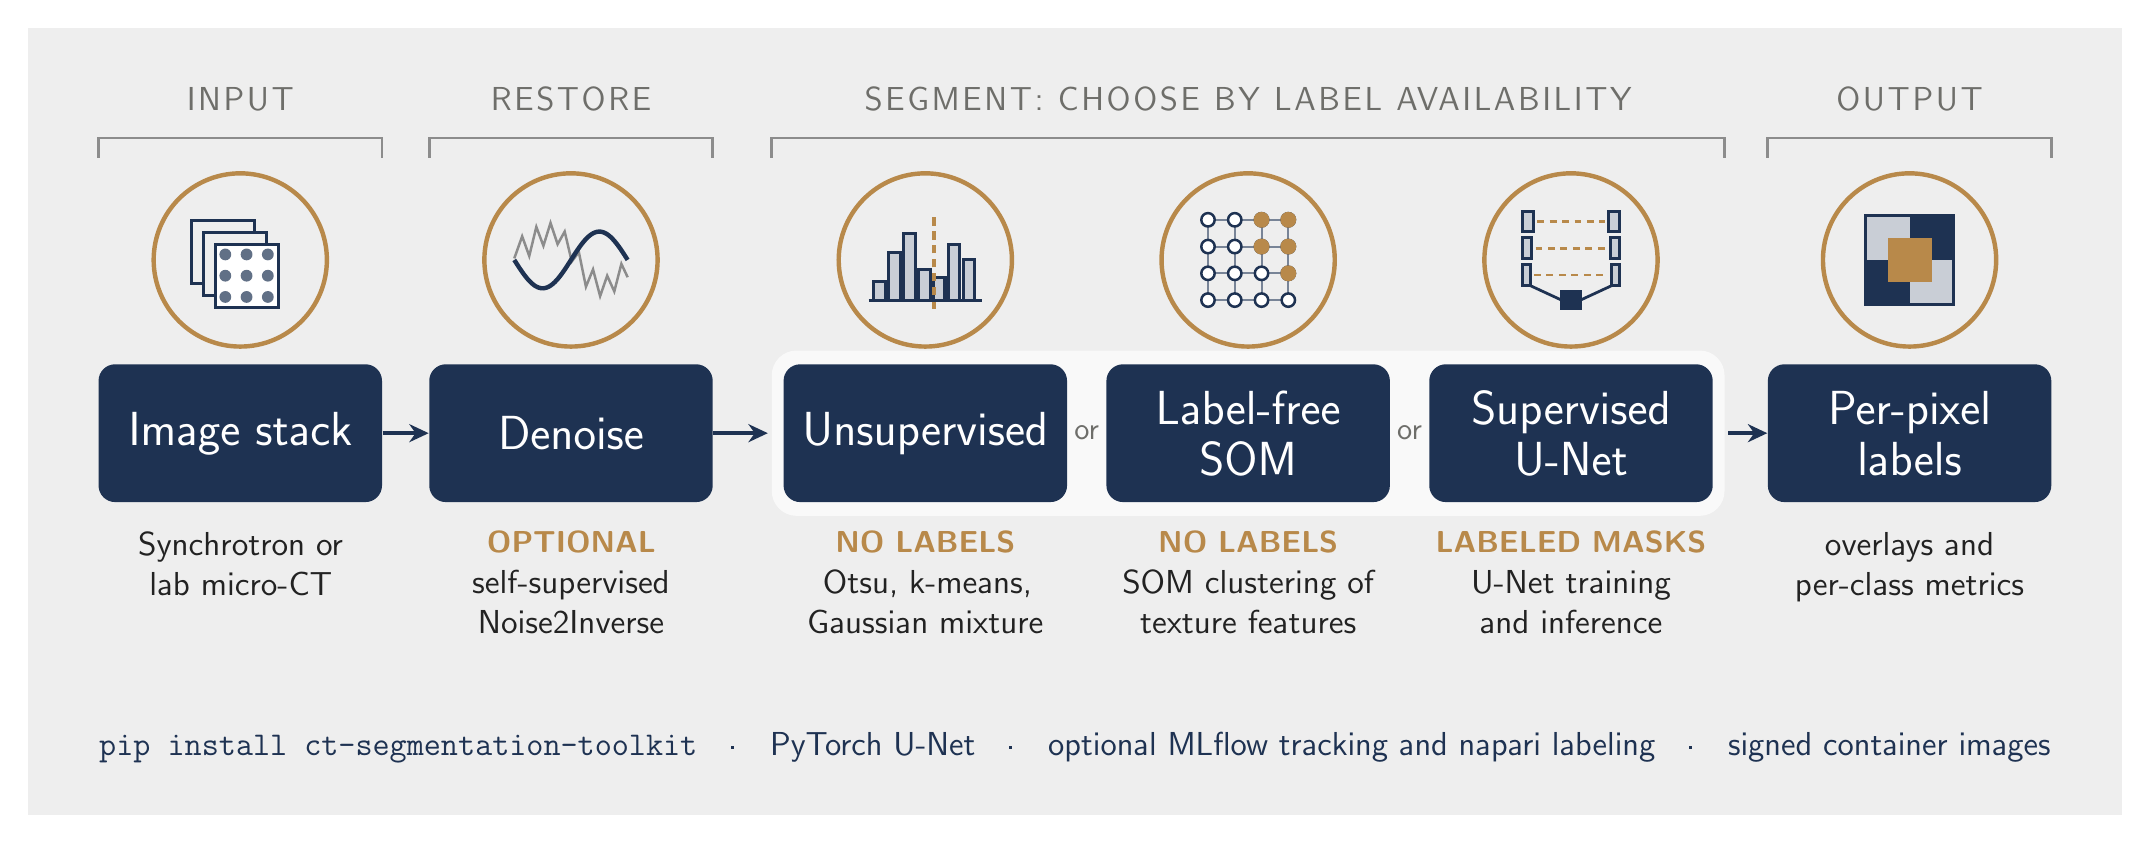
\begin{tikzpicture}[x=1cm,y=1cm]

% ---- page -------------------------------------------------------------------------------
\fill[page] (0,0) rectangle (26.6,10);

% ---- column centres (x) and fixed row bands (y) -------------------------------------------
%  input 2.7 | restore 6.9 | segment 11.4 / 15.5 / 19.6 | output 23.9
\def\yring{7.05}   % icon ring centres (ring spans 5.95-8.15)
\def\ybox{4.85}    % stage box centres (box spans 3.975-5.725)
\def\ycap{3.72}    % caption tops

% ---- phase brackets -----------------------------------------------------------------------
\phasebracket{0.9}{4.5}{INPUT}
\phasebracket{5.1}{8.7}{RESTORE}
\phasebracket{9.45}{21.55}{SEGMENT: CHOOSE BY LABEL AVAILABILITY}
\phasebracket{22.1}{25.7}{OUTPUT}

% ---- icon rings -----------------------------------------------------------------------------
\foreach \x in {2.7,6.9,11.4,15.5,19.6,23.9} \node[ring] at (\x,\yring) {};

% Icon 1 -- image stack: three offset slices; the front slice shows rod cross-sections.
\begin{scope}[shift={(2.7,\yring)}]
  \draw[ico, fill=page] (-0.62,-0.30) rectangle (0.18,0.50);
  \draw[ico, fill=page] (-0.47,-0.45) rectangle (0.33,0.35);
  \draw[ico, fill=white] (-0.32,-0.60) rectangle (0.48,0.20);
  \foreach \i in {0,1,2} \foreach \j in {0,1,2}
    \fill[navy!70] ({-0.19+\i*0.27},{-0.47+\j*0.27}) circle (0.075);
\end{scope}

% Icon 2 -- denoising: a noisy trace (grey) and the recovered smooth signal (navy).
\begin{scope}[shift={(6.9,\yring)}]
  \draw[rule, line width=0.9pt] plot[smooth, tension=0] coordinates {
    (-0.72,0.02) (-0.62,0.30) (-0.53,0.05) (-0.44,0.42) (-0.35,0.18) (-0.26,0.47)
    (-0.17,0.20) (-0.08,0.36) (0.01,-0.02) (0.10,0.10) (0.19,-0.34) (0.28,-0.12)
    (0.37,-0.46) (0.46,-0.20) (0.55,-0.40) (0.64,-0.05) (0.72,-0.22)};
  \draw[navy, line width=1.6pt, domain=-0.72:0.72, samples=60, smooth]
    plot (\x, {0.36*sin(250*\x)});
\end{scope}

% Icon 3 -- intensity clustering: a two-population histogram split by thresholds.
\begin{scope}[shift={(11.4,\yring)}]
  \foreach \i/\h in {0/0.25,1/0.62,2/0.85,3/0.40,4/0.30,5/0.72,6/0.52}
    \draw[ico, fill=tone] ({-0.66+\i*0.19},-0.52) rectangle ++(0.15,\h);
  \draw[gold, line width=1.3pt, dash pattern=on 3pt off 2pt] (0.11,-0.62) -- (0.11,0.55);
  \draw[ico] (-0.72,-0.52) -- (0.72,-0.52);
\end{scope}

% Icon 4 -- self-organizing map: a 4 x 4 node lattice; one cluster of nodes highlighted.
\begin{scope}[shift={(15.5,\yring)}]
  \foreach \i in {0,...,3} {
    \draw[navy!60, line width=0.7pt] ({-0.51+\i*0.34},-0.51) -- ({-0.51+\i*0.34},0.51);
    \draw[navy!60, line width=0.7pt] (-0.51,{-0.51+\i*0.34}) -- (0.51,{-0.51+\i*0.34}); }
  \foreach \i in {0,...,3} \foreach \j in {0,...,3}
    \filldraw[navy, fill=white, line width=0.9pt] ({-0.51+\i*0.34},{-0.51+\j*0.34}) circle (0.085);
  \foreach \i/\j in {2/2,3/2,2/3,3/3,3/1}
    \filldraw[gold, line width=0.9pt] ({-0.51+\i*0.34},{-0.51+\j*0.34}) circle (0.085);
\end{scope}

% Icon 5 -- U-Net: encoder blocks down, decoder blocks up, dashed skip connections.
\begin{scope}[shift={(19.6,\yring)}]
  \foreach \y/\w in {0.36/0.14,0.02/0.12,-0.32/0.10}{
    \draw[ico, fill=tone] ({-0.62},{\y}) rectangle ++(\w,0.26);
    \draw[ico, fill=tone] ({0.62-\w},{\y}) rectangle ++(\w,0.26);
    \draw[gold, line width=1pt, dash pattern=on 2.5pt off 2pt] ({-0.62+\w+0.05},{\y+0.13}) -- ({0.62-\w-0.05},{\y+0.13}); }
  \draw[ico, fill=navy] (-0.12,-0.62) rectangle (0.12,-0.40);
  \draw[navy, line width=1pt] (-0.53,-0.32) -- (-0.12,-0.51);
  \draw[navy, line width=1pt] (0.53,-0.32) -- (0.12,-0.51);
\end{scope}

% Icon 6 -- label map: a small mask with three classes.
\begin{scope}[shift={(23.9,\yring)}]
  \foreach \i/\j/\c in {0/0/navy,1/0/navy,2/0/tone,3/0/tone, 0/1/navy,1/1/gold,2/1/gold,3/1/tone,
                        0/2/tone,1/2/gold,2/2/gold,3/2/navy, 0/3/tone,1/3/tone,2/3/navy,3/3/navy}
    \fill[\c] ({-0.56+\i*0.28},{-0.56+\j*0.28}) rectangle ++(0.28,0.28);
  \draw[ico] (-0.56,-0.56) rectangle (0.56,0.56);
\end{scope}

% ---- the choose-one panel behind the three segmentation routes ----------------------------
\fill[white, rounded corners=9pt, opacity=0.65] (9.45,3.8) rectangle (21.55,5.9);
\node[text=phase, font=\fontsize{11}{13}\selectfont] at (13.45,\ybox) {or};
\node[text=phase, font=\fontsize{11}{13}\selectfont] at (17.55,\ybox) {or};

% ---- stage boxes ------------------------------------------------------------------------------
\node[stage] (in)  at (2.7,\ybox)  {Image stack};
\node[stage] (dn)  at (6.9,\ybox)  {Denoise};
\node[stage] (uns) at (11.4,\ybox) {Unsupervised};
\node[stage] (som) at (15.5,\ybox) {Label-free\\SOM};
\node[stage] (sup) at (19.6,\ybox) {Supervised\\U-Net};
\node[stage] (out) at (23.9,\ybox) {Per-pixel\\labels};

% ---- flow arrows: into and out of the panel, never through the alternatives ---------------
\draw[flow] (in.east) -- (dn.west);
\draw[flow] (dn.east) -- (9.4,\ybox);
\draw[flow] (21.6,\ybox) -- (out.west);

% ---- captions (fixed band under the boxes) ---------------------------------------------------
\node[capt] at (2.7,\ycap)  {Synchrotron or\\lab micro-CT};
\node[capt] at (6.9,\ycap)  {\textcolor{gold}{\bfseries\fontsize{10.5}{12.5}\selectfont OPTIONAL}\\self-supervised\\Noise2Inverse};
\node[capt] at (11.4,\ycap) {\textcolor{gold}{\bfseries\fontsize{10.5}{12.5}\selectfont NO LABELS}\\Otsu, k-means,\\Gaussian mixture};
\node[capt] at (15.5,\ycap) {\textcolor{gold}{\bfseries\fontsize{10.5}{12.5}\selectfont NO LABELS}\\SOM clustering of\\texture features};
\node[capt] at (19.6,\ycap) {\textcolor{gold}{\bfseries\fontsize{10.5}{12.5}\selectfont LABELED MASKS}\\U-Net training\\and inference};
\node[capt] at (23.9,\ycap) {overlays and\\per-class metrics};

% ---- footer ---------------------------------------------------------------------------------------
\node[text=navy, font=\fontsize{12}{14.5}\selectfont] at (13.3,0.85)
  {\texttt{pip install ct-segmentation-toolkit}\quad\textperiodcentered\quad PyTorch U-Net\quad\textperiodcentered\quad
   optional MLflow tracking and napari labeling\quad\textperiodcentered\quad signed container images};

\end{tikzpicture}
\end{document}
